\subsection{Elastix - Open Source Unified Communications Server}

Esta ferramenta é um software livre, que integra as seguintes funcionalidades(figura~\ref{fig:elastix}):
\begin{itemize}
\item VoIP PBX
\item Fax
\item Instant Messsaging
\item Mail Server
\item Video Conference
\end{itemize}

\begin{figure}[H]
    \begin{center}
        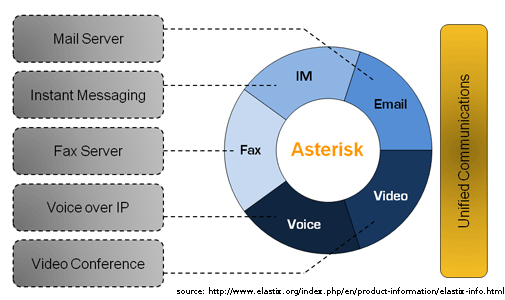
\includegraphics[width=12cm]{include/img/elastix.png}
    \end{center}
    \caption{Estrutura de Elastix}
    \label{fig:elastix}
\end{figure}

A sua principal funcionalidade, é permitir ao utilizador configurar de uma forma mais simples uma 
central de telefonia VoIP, usando como software o \emph{Asterisk(Free PBX)}. O Elastix é acedido através de uma plataforma
web que pode ser acedida atráves do seguinte endereço \emph{https://<IP\_DO\_SERVIDOR>}, figura~\ref{fig:elastix_login}.

\begin{figure}[H]
    \begin{center}
        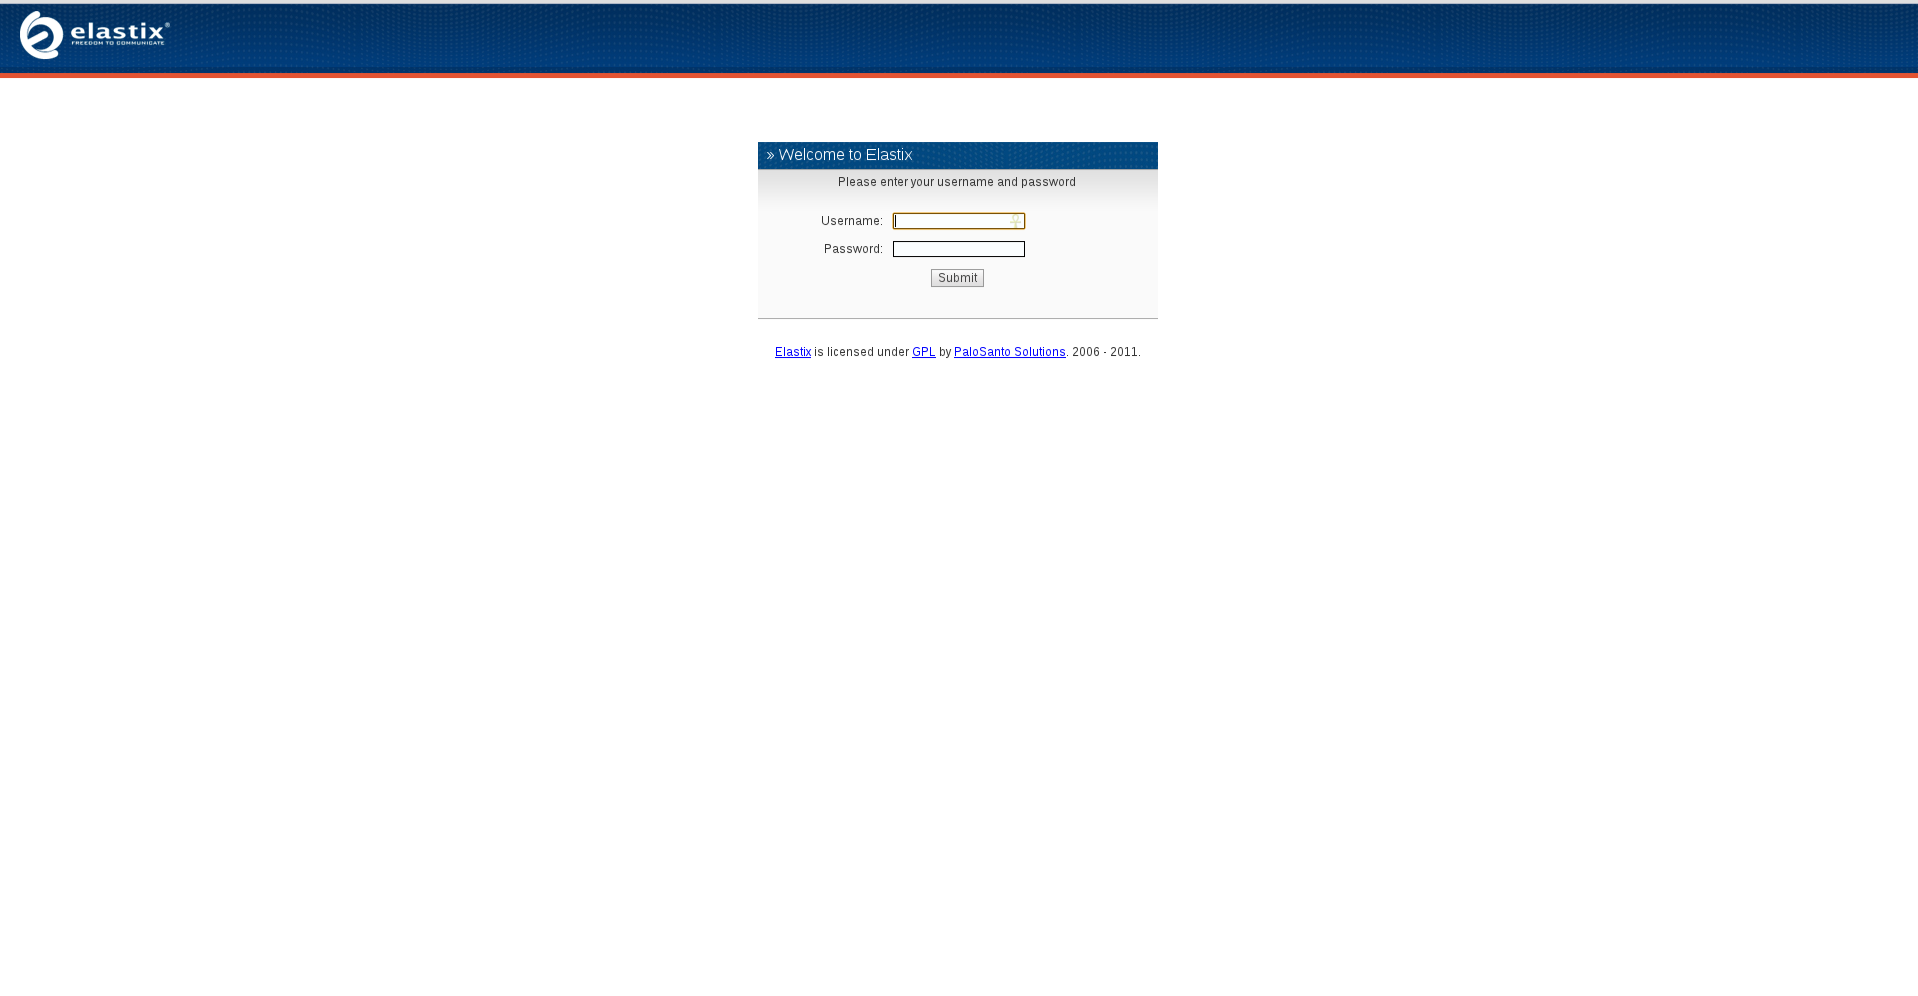
\includegraphics[width=13cm]{include/img/elastix_login.png}
    \end{center}
    \caption{Elastix Login}
    \label{fig:elastix_login}
\end{figure}

Após se efectuar o login na plataforma web, podemos aceder ao Free PBX(figura~\ref{fig:elastix_pbx_extensions}) e a partir
desse momento, podemos configurar tudo o que é necessário para que uma central telefônica VoIP funcione correctamente, tais como \emph{extensões telefônicas\footnote{Local onde se configura as extensões telefônicas, que posteriormente serão configuradas nos telefones VoIP}}, \emph{Trunks}(figura~\ref{fig:elastix_pbx_trunk}), \emph{Outbound Routes\footnote{Onde se configura as rotas de saida para as chamadas telefônicas}}(figura~\ref{fig:elastix_pbx_outboundRoutes}) e \emph{Inbound Routes\footnote{Onde se configura as rotas de entrada, definindo os telefones responsáveis por receber as chamadas do exterior}}.

\begin{figure}[H]
    \begin{center}
        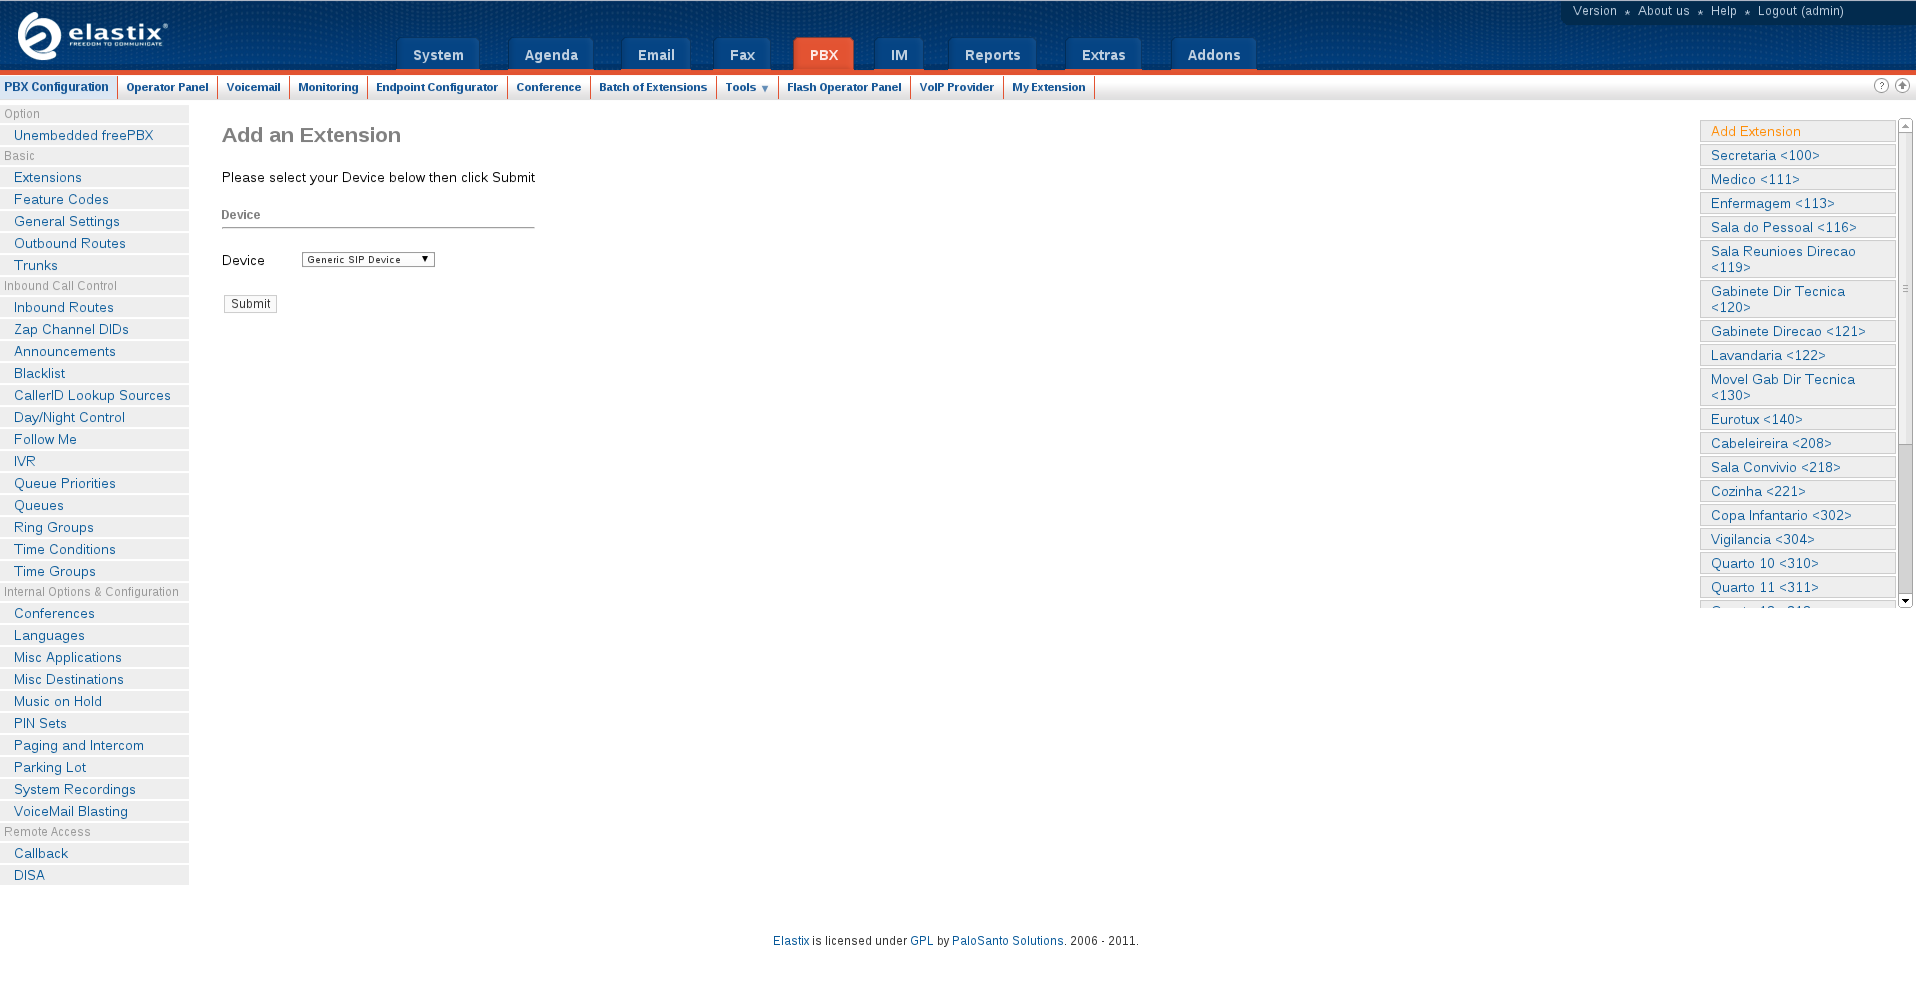
\includegraphics[width=13cm]{include/img/elastix_pbx_extensions.png}
    \end{center}
    \caption{Elastix Extensions}
    \label{fig:elastix_pbx_extensions}
\end{figure}

\begin{figure}[H]
    \begin{center}
        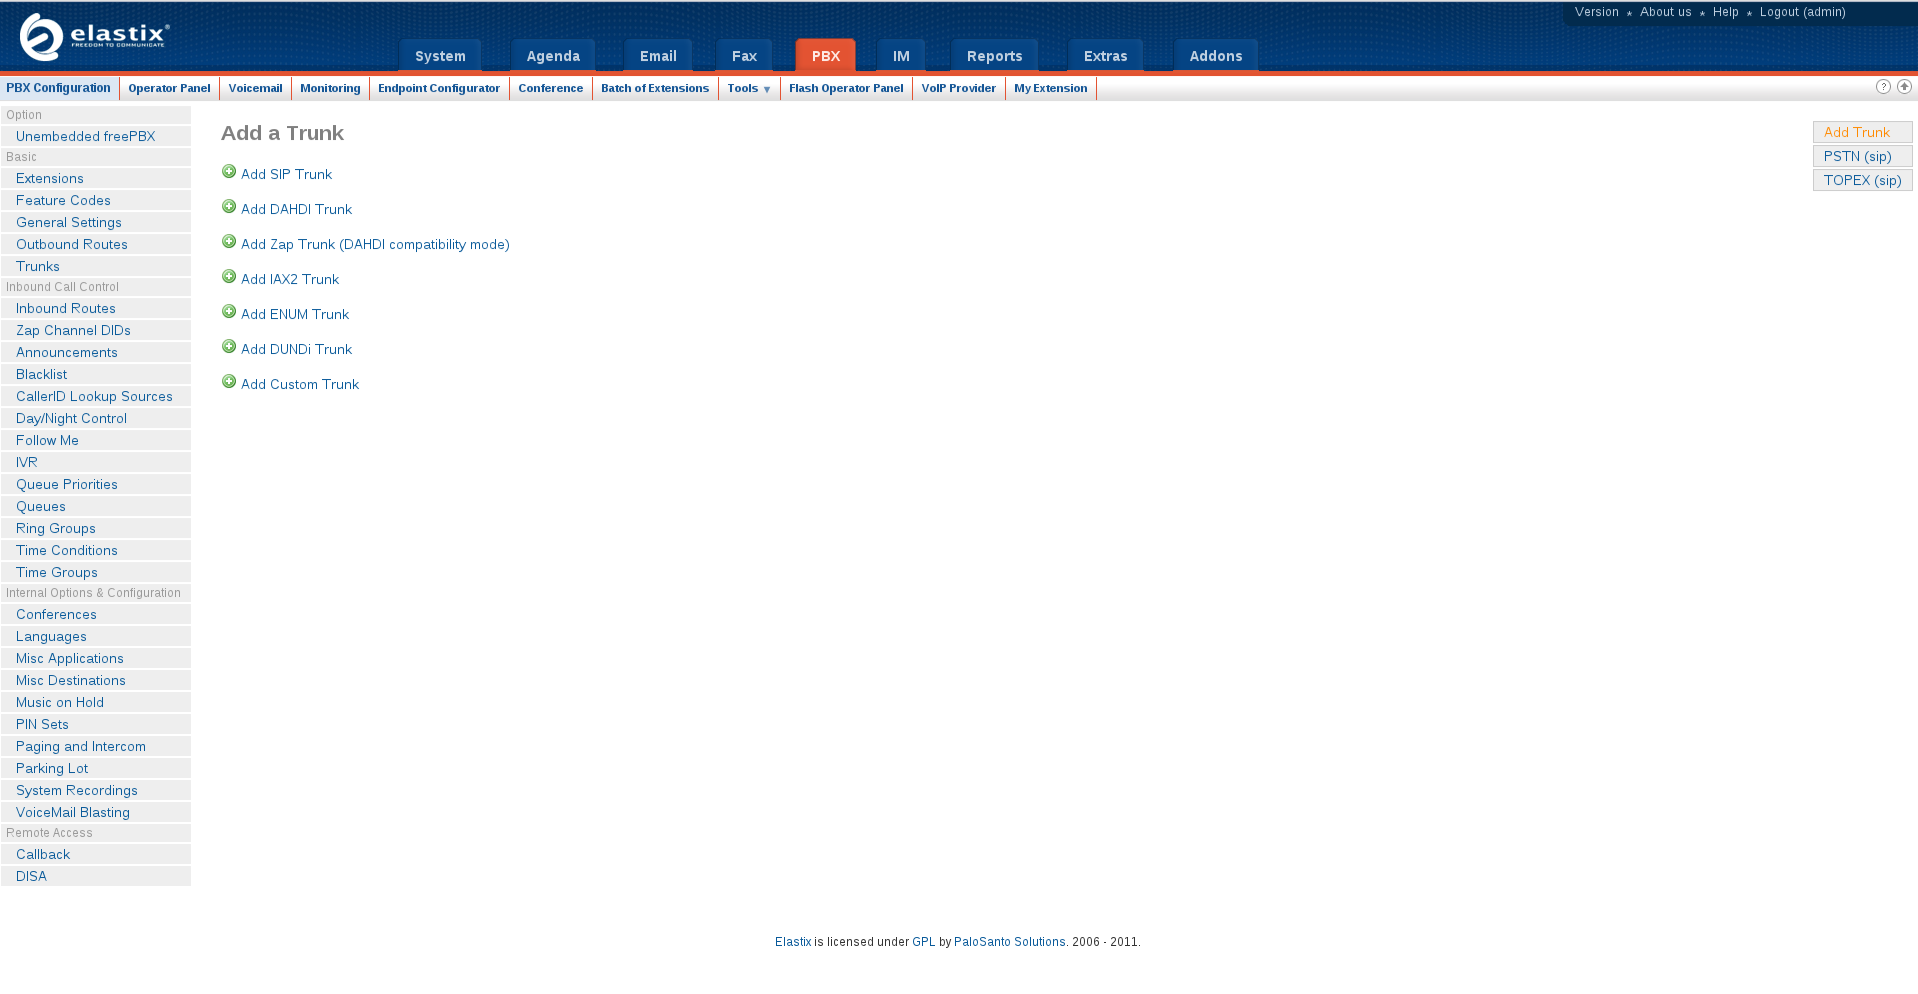
\includegraphics[width=13cm]{include/img/elastix_pbx_trunk.png}
    \end{center}
    \caption{Elastix Trunks}
    \label{fig:elastix_pbx_trunk}
\end{figure}

\begin{figure}[H]
    \begin{center}
        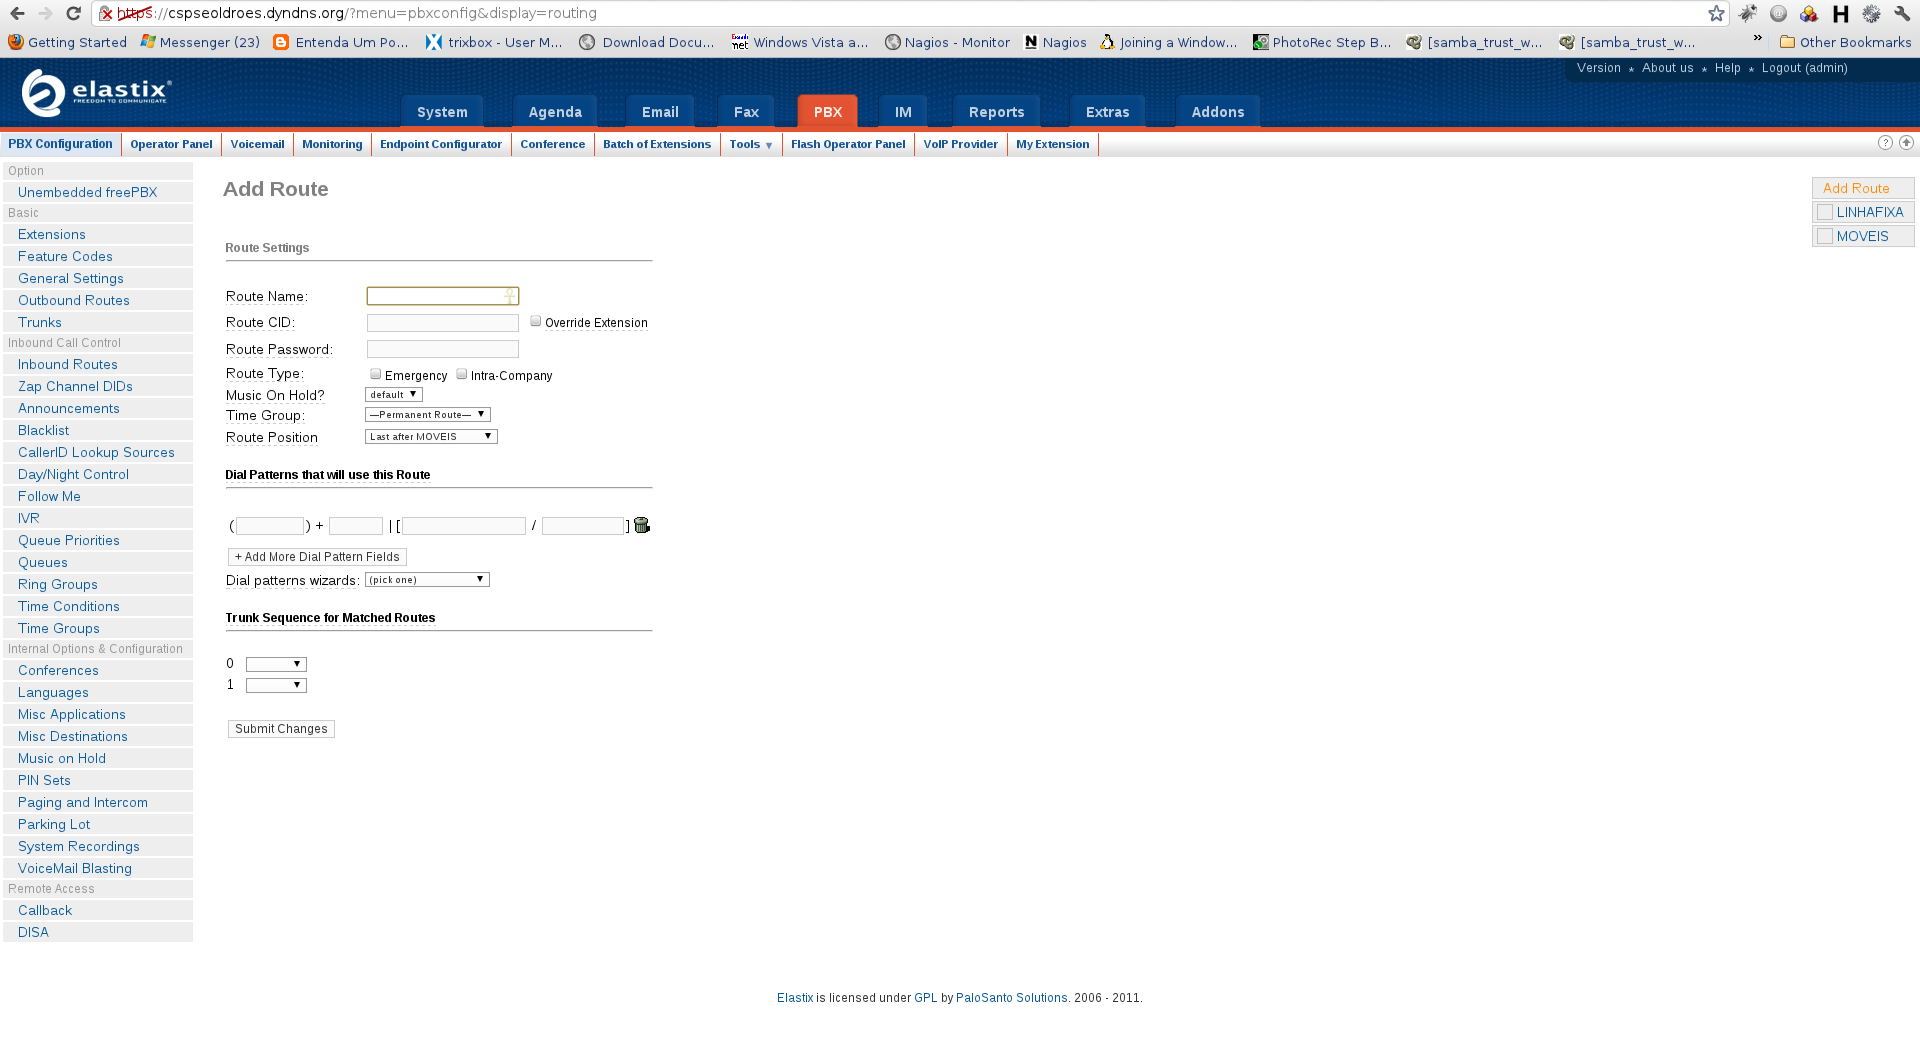
\includegraphics[width=13cm]{include/img/elastix_pbx_outboundRoutes.png}
    \end{center}
    \caption{Elastix outbound Routes}
    \label{fig:elastix_pbx_outboundRoutes}
\end{figure}


Para mais informações, pode aceder aos manuais do produto no seguinte endereço: \begin{normalsize}\sffamily\href{http://www.elastix.org/index.php/en/product-information/manuals-books.html}{www.elastix.org/index.php/en/product-information/manuals-books.html}\end{normalsize}
